\section{Build systems}

\begin{frame}
    \frametitle{Makefile}

    \begin{figure}[H]
        \centering
        \hfill
        \begin{minipage}{.95\textwidth}
            \inputminted[
                mathescape,
                linenos,
                autogobble,
                fontsize=\tiny,
            ]{makefile}{E:\\GitHub\\presentation_in_LaTeX\\c_project_development\\proj\\auto_proj_2\\Makefile}
        \end{minipage}
        \hfill
        \caption*{Example of a Makefile with build and clean targets.}
    \end{figure}
\end{frame}

\begin{frame}
    \frametitle{Makefile compile}

    \begin{figure}[H]
        \centering
        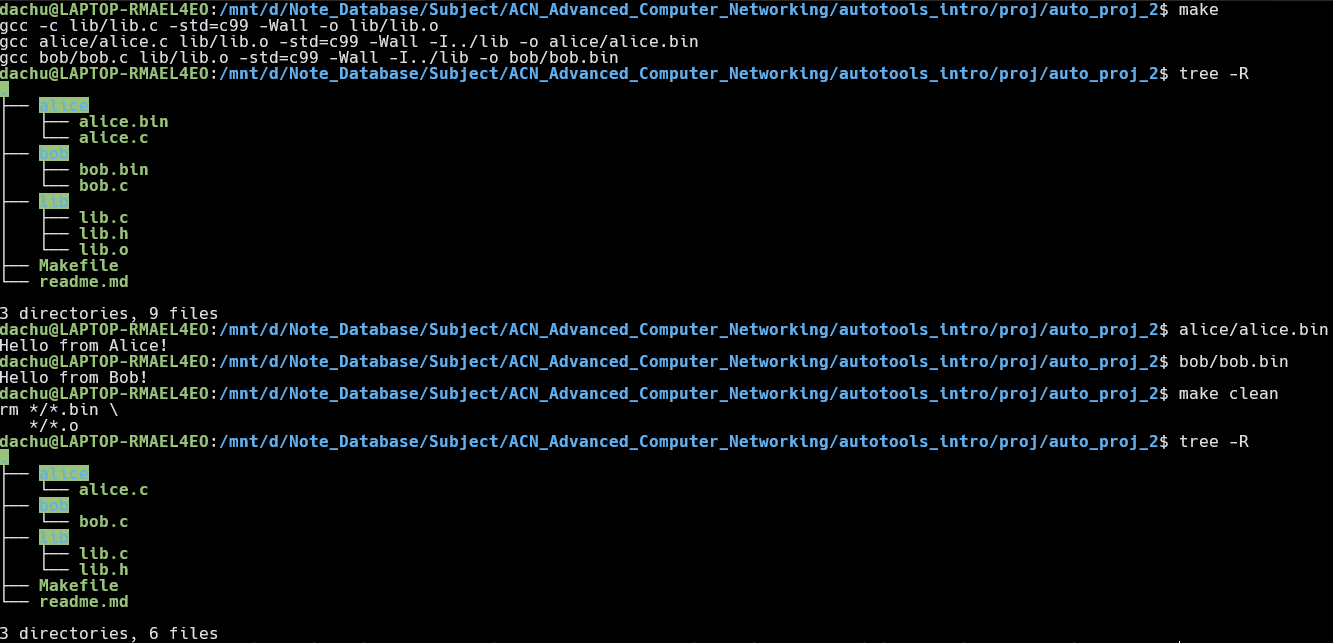
\includegraphics[width=0.9\textwidth]{../figure/makefile_compile.png}
        \caption*{Tree structure and execution results after compilation.}
    \end{figure}
\end{frame}

\begin{frame}
    \frametitle{Makefile}

    \begin{itemize}
        \item Work similar to \textit{Bash}
        \item Can specify a single target with all of its dependency compiled
        \item Takes a lot of time to configure if there are too many files
        \item All actions include \alert{building}, \alert{installing}, \alert{uninstalling}, and \alert{clearing} require knowledge of convension and manual configuration
    \end{itemize}
\end{frame}

\begin{frame}
    \frametitle{Development pipeline with build systems}

    \begin{center}
        \begin{tikzpicture}[node distance=2cm]
            \node (start) [block] {\textit{C} project};
            \node (bs1) [block, below of=start] {Autotools/make};
            \node (bs2) [block, left of=bs1, xshift=-1cm] {CMake/make};
            \node (bs3) [block, right of=bs1, xshift=1cm] {Meson/ninja};
            \node (f) [block, below of=bs1] {\texttt{bin *.o *.a *.so *.so.x.x.x *.conf *.d *.x (man) *.h *.pc}};
            \node (def) [path, below of=f, xshift=-3cm] {base dir: \texttt{/usr} or \texttt{/usr/local}\\
                \texttt{/usr/bin}\\
                \texttt{/usr/lib}\\
                \texttt{/usr/include}\\
                $\cdots$};
            \node (gen) [path, below of=f, xshift=3cm] {base dir: \texttt{/custom/path}\\
                \texttt{/custom/path/bin}\\
                \texttt{/custom/path/lib}\\
                \texttt{/custom/path/include}\\
                $\cdots$};

            \draw [arrow] (start) -- (bs1);
            \draw [arrow] (start) -- (bs2);
            \draw [arrow] (start) -- (bs3);
            \draw [arrow] (bs1) -- (f);
            \draw [arrow] (bs2) -- (f);
            \draw [arrow] (bs3) -- (f);
            \draw [arrow] (f) -- (def);
            \draw [arrow] (f) -- (gen);
        \end{tikzpicture}
    \end{center}
\end{frame}

\begin{frame}
    \frametitle{Why build systems}

    \begin{itemize}
        \item Dependency checks on existence and version (pkg-config)
        \item Multi-platform portability (\texttt{config.h} and \texttt{./configure})
        \item Standardized build process
        \item Standardized convensions (like \texttt{./configure --prefix=/path --exec-path=/path})
        \item Incremental build, which only build changed files
        \item Library management (\texttt{libtool})
        \item Run tests after compilation if existed
    \end{itemize}
\end{frame}

\begin{frame}
    \frametitle{Common build systems}

    \begin{center}
        \footnotesize
        \begin{tabular}{ c | c c c }
            \hline
            Build system & Autotools/make & CMake/make & Meson/ninja \\
            \hline
            Common usecase & GNU libraries & \textit{C++} projects & GNOME \\
            \hline
            Common files & \texttt{configure.ac} & \texttt{CMakeLists.txt} & \texttt{meson.build} \\
            to identify & \texttt{Makefile.am} & & \texttt{meson.options} \\
            \hline
            \multirow[t]{6}{*}{Build command} & \scriptsize\texttt{cd \$project\_dir} & \scriptsize\texttt{cd \$project\_dir} & \scriptsize\texttt{cd \$project\_dir} \\
            & \scriptsize\texttt{./configure} & \scriptsize\texttt{mkdir build} & \scriptsize\texttt{meson setup \_build} \\
            & \scriptsize\texttt{make} & \scriptsize\texttt{cd build} & \scriptsize\texttt{meson compile -C \_build} \\
            & \scriptsize\texttt{make install} & \scriptsize\texttt{cmake ..} & \scriptsize\texttt{meson install -C \_build} \\
            & & \scriptsize\texttt{make} & \\
            & & \scriptsize\texttt{make install} & \\
            \hline
        \end{tabular}
    \end{center}
\end{frame}
